\documentclass[11pt,a4paper]{article}
\usepackage[margin=25mm]{geometry}
\usepackage{amsmath,amssymb,amsthm,bm,mathtools}
\usepackage[T1]{fontenc}
\usepackage{lmodern,microtype}
\usepackage{graphicx}
\usepackage{booktabs}
\usepackage{array}
\usepackage{enumitem}
\usepackage[colorlinks=true,linkcolor=blue,urlcolor=blue,citecolor=blue]{hyperref}
\newcommand{\R}{\mathbb R}
\newcommand{\E}{\mathbb E}
\newcommand{\tr}{\operatorname{tr}}
\newcommand{\col}{\operatorname{col}}
\newcommand{\sX}{\hat s_X^2}
\newcommand{\sY}{\hat s_Y^2}
\newcommand{\amp}{\mathcal A}
\newcommand{\task}{\textsf{[task]}}
\newcommand{\prior}{\textsf{[prior]}}
\newcommand{\mixed}{\textsf{[task $\times$ prior]}}
\newtheorem{lemma}{Lemma}
\newtheorem{proposition}{Proposition}
\theoremstyle{remark}
\newtheorem{remark}{Remark}
\title{Limiting cases of the one-hidden-layer linear solution\\and the spatial scale of functional cell types}
\author{}
\date{}
\begin{document}
\maketitle

\begin{abstract}
We re-derive the implicit solution \texttt{eq:linear-soln} of Section~2 for a linear network with one spatially embedded hidden layer, and find that it agrees with the proofread (red) form of the notes; the whole analysis below therefore refers to that corrected equation. Per data mode, the hidden-layer variance at spatial frequency $q$ factorises as a prior-shaped, rate-penalty-shrunk variance times a target-driven amplification, $d_q = \pi_q \amp_q$, and $d_q$ is monotone in $\lambda_q$: every data mode is smoothest at $q = 0$, so spatial ``cell types'' can only appear in the \emph{ratios} of the spectra of different data modes. We work out the limits $\sigma \to 0$, $r \to 0$, $k_0 = k_1$, a Gaussian kernel on a ring, and the uniform latent task, and identify three mechanisms that move the spatial scale of one latent relative to another: the input-noise floor (no effect on shape at weak target), rate-penalty whitening (a strong latent is pushed to \emph{finer} scales), and target condensation (a strong latent is pushed to \emph{coarser} scales, up to the system size). In the uniform-$[0,a]$ task the ``strong latent'' is always the mean direction $\sum_k z_k$, whose singular value exceeds the $K-1$ degenerate contrast directions by $3K+1$; individual latents are not identifiable. Eight numerical predictions close the note. Every non-trivial step is checked in \path{latex/notes/scripts/check_linear_soln_limits.py}.
\end{abstract}

\section*{Summary of conclusions}
\addcontentsline{toc}{section}{Summary of conclusions}
\begin{itemize}[nosep]
  \item The re-derivation reproduces the corrected \texttt{eq:linear-soln}; the ansatz is an exact fixed point of the full map when $[XX^\top, YY^\top] = 0$ (machine precision against an ansatz-free Newton solve), and off by $\sim0.2\%$ for a mildly non-orthonormal teacher.
  \item $d_q = \pi_q\amp_q$ (prior-shrunk variance times target amplification) is monotone in $\lambda_q$: no data mode peaks at an intermediate spatial frequency; spatial cell types are relative statements between data modes, and at $\sigma = r = 0$, $\delta = 0$ (or weak targets) all data modes of the latent task share one profile.
  \item $\sigma$ adds a white floor and, at weak target, nothing else; $r$ caps and \emph{whitens} strong modes; $\beta$ (through $\delta$) \emph{condenses} strong modes onto $q = 0$ with correlation length $\propto\hat s_Y$ (no true condensate in $d\le2$ for $N\to\infty$); a common $k_0 = k_1$ is a gain knob with maximal target effect at $k_* = \sqrt{m/(\kappa s_X^2\bar\lambda_2)}$.
  \item In the uniform-$[0,a]$ task the strong mode is the mean direction ($s_1^2/s_k^2 = 3K+1$); the contrasts are degenerate and individual latents are not identifiable by the linear theory.
\end{itemize}

\tableofcontents

\section{Starting point}
\label{sec:start}

\subsection{Model and assumptions}
One hidden layer of $N$ linear units on a periodic lattice, $h^{\mu}_i = \phi^{\mu}_i$, with $P$ patterns $\mu$, $m$ inputs $a$ and $n$ outputs $\alpha$; the readout is $f^\mu_\alpha = N^{-1}\sum_j W^{(1)}_{\alpha,j}\phi^\mu_j$ and the first layer carries Gaussian input noise of variance $\sigma^2$.
Priors (Section~2 of the notes): $K^{(0),\mathrm{post}} = K^{(1),\mathrm{pre}} \equiv K$ is a real, symmetric, translation-invariant $N\times N$ kernel, $K^{(0),\mathrm{pre}} = k_0 I_m$, $K^{(1),\mathrm{post}} = k_1 I_n$, and the rate penalty is $G = r I_N$. The loss prefactor and temperature give $\kappa = \beta/(Pn)$ and the ridge $\delta = 1/(k_1\kappa) = Pn/(\beta k_1)$.
Throughout, $F$ is the unitary discrete Fourier matrix, $F_{i,q} = N^{-1/2} e^{2\pi \mathrm i q i/N}$, $q \in \{-N/2+1,\dots,N/2\}$, and $K = F\Lambda F^\dagger$ with real eigenvalues $\lambda_q = \lambda_{-q} \ge 0$; we write $\lambda_0 = \max_q \lambda_q$ (true for every kernel that decreases with distance) and $\bar\lambda = \frac1N\sum_q\lambda_q = K_{i,i}$.
Data: $A = \frac{k_0}{m} XX^\top$ and $YY^\top$ ($P\times P$); the mutual-diagonalisability ansatz is $XX^\top = U S_X^2 U^\top$, $YY^\top = U S_Y^2 U^\top$ with one orthogonal $U$, which requires $[XX^\top, YY^\top] = 0$. Per data mode $p$ we write $s_X^2, s_Y^2$ for the diagonal entries and
\begin{equation}
  \sX = \frac{k_0 s_X^2}{m}, \qquad \sY = \frac{s_Y^2}{k_1}, \qquad \delta = \frac{1}{k_1\kappa} .
\end{equation}

\subsection{Re-derivation from the single-site distribution}
\label{sec:rederive}

\begin{lemma}[Gaussian single site]\label{lem:gauss}
With the rotated conjugate $\hat\Phi$, the single-site distribution of the hidden layer is Gaussian in $h \in \R^{P\times N}$ with precision
\begin{equation}
  \mathcal P = (A\otimes K + \sigma^2 I)^{-1} - (B\otimes K - r I),
  \qquad (M\otimes K)^{\mu,\nu}_{i,j} = M^{\mu,\nu}K_{i,j},
  \label{eq:precision}
\end{equation}
where $B^{\mu,\nu} = K^{(1),\mathrm{post}}_{\alpha,\beta}\hat\Phi^{\mu,\nu}_{\alpha,\beta}$. The integral exists iff $\mathcal P \succ 0$, and then $\langle h^\mu_i h^\nu_j\rangle = (\mathcal P^{-1})^{\mu,\nu}_{i,j}$.
\end{lemma}
\begin{proof}
The input kernel is $\Phi^{(0)\mu,\nu}_{i,j} = \frac1m x^\mu_a K^{(0)}_{i,a,j,b} x^\nu_b = \frac{k_0}{m}(XX^\top)^{\mu,\nu}K_{i,j}$ and the noise adds $\sigma^2\delta^{\mu,\nu}\delta_{i,j}$ (\texttt{eq:single-site-reg}); the tilt is $\frac12\phi^\mu_i(\hat\Phi^{\mu,\nu}_{\alpha,\beta}K^{(1)}_{\alpha,i,\beta,j} - G_{i,j}\delta^{\mu,\nu})\phi^\nu_j$ with $K^{(1)}_{\alpha,i,\beta,j} = k_1\delta_{\alpha,\beta}K_{i,j}$, which is $\frac12\phi(B\otimes K - rI)\phi$. With $\phi = h$ the exponent is $-\frac12 h^\top\mathcal P h$.
\end{proof}

\begin{lemma}[Fourier block-diagonalisation]\label{lem:fourier}
$\mathcal P = \sum_q (f_q f_q^\dagger)\otimes\Sigma_q^{-1}$ with $f_q$ the $q$-th column of $F$ and
\begin{equation}
  \Sigma_q^{-1} = (\lambda_q A + \sigma^2 I_P)^{-1} - (\lambda_q B - r I_P) .
  \label{eq:sigma-q}
\end{equation}
Hence $\mathcal P \succ 0$ iff $\Sigma_q^{-1}\succ0$ for every $q$, and $\langle h^\mu_i h^\nu_j\rangle = \sum_q F_{i,q}\Sigma_q^{\mu,\nu}F^*_{j,q}$.
\end{lemma}
\begin{proof}
$A\otimes K + \sigma^2 I = \sum_q f_qf_q^\dagger\otimes(\lambda_q A + \sigma^2 I)$ because $K = \sum_q\lambda_q f_qf_q^\dagger$ and $I_N = \sum_q f_qf_q^\dagger$; the $f_qf_q^\dagger$ are orthogonal projectors, so the inverse acts blockwise. The same decomposition applies to $B\otimes K - r I$.
\end{proof}

\begin{lemma}[Hidden-layer kernel]\label{lem:C}
$C^{\mu,\nu} = \frac1N\sum_{i,j}K_{i,j}\langle h^\mu_i h^\nu_j\rangle = \frac1N\sum_q\lambda_q\Sigma_q^{\mu,\nu}$.
\end{lemma}
\begin{proof}
$\sum_{i,j}K_{i,j}F_{i,q}F^*_{j,q} = (F^\dagger K F)_{q,q}$ when $K$ is symmetric, and $F^\dagger KF = \Lambda$. The $1/N$ is the one in \texttt{eq:kernel-def} (see \path{rg_kernel_normalisation.tex}).
\end{proof}

\begin{lemma}[Readout tilt]\label{lem:B}
$\Phi^{(1)} = k_1 I_n\otimes C$, $\hat\Phi^{(1)} = \tilde\Phi^{-1}\mathbb Y\tilde\Phi^{-1}$ with $\tilde\Phi = \Phi^{(1)} + \kappa^{-1}I$, and therefore
\begin{equation}
  B = \frac1{k_1}\tilde C^{-1}YY^\top\tilde C^{-1}, \qquad \tilde C = C + \delta I_P .
\end{equation}
\end{lemma}
\begin{proof}
$\tilde\Phi = k_1 I_n\otimes(C + \delta I_P)$, so $\tilde\Phi^{-1} = k_1^{-1}I_n\otimes\tilde C^{-1}$ and, with $\mathbb Y^{\mu,\nu}_{\alpha,\beta} = y^\mu_\alpha y^\nu_\beta$, $\hat\Phi^{\mu,\nu}_{\alpha,\beta} = k_1^{-2}[\tilde C^{-1}]^{\mu,\mu'}y^{\mu'}_\alpha y^{\nu'}_\beta[\tilde C^{-1}]^{\nu',\nu}$ (summed over the pattern indices $\mu',\nu'$). Contracting with $K^{(1),\mathrm{post}}_{\alpha,\beta} = k_1\delta_{\alpha,\beta}$ sums $y^{\mu'}_\alpha y^{\nu'}_\alpha$ over $\alpha$ into $(YY^\top)^{\mu',\nu'}$ and leaves one factor $k_1^{-1}$.
\end{proof}

\begin{lemma}[Ansatz reduction]\label{lem:ansatz}
Let $XX^\top = US_X^2U^\top$ and $YY^\top = US_Y^2U^\top$. If $\tilde C = UD_CU^\top$ then every $\Sigma_q = UD_qU^\top$ and the updated $\tilde C$ of Lemma~\ref{lem:C} is again diagonal in $U$; the family of $U$-diagonal $\tilde C$ is invariant under the fixed-point map. Per data mode, with $c$ the diagonal entry of $D_C$,
\begin{equation}
  d_q^{-1} = \frac{1}{\lambda_q\sX + \sigma^2} + r - \frac{\lambda_q\sY}{c^2},
  \qquad
  c = \delta + \frac1N\sum_q\lambda_q d_q .
  \label{eq:per-mode}
\end{equation}
\end{lemma}
\begin{proof}
In \eqref{eq:sigma-q}, $\lambda_qA + \sigma^2 I = U(\lambda_q\frac{k_0}{m}S_X^2 + \sigma^2I)U^\top$ and $\lambda_qB - rI = U(\frac{\lambda_q}{k_1}D_C^{-2}S_Y^2 - r I)U^\top$, both diagonal; so is their difference and its inverse. $\tilde C = \frac1N\sum_q\lambda_q UD_qU^\top + \delta I$ is diagonal in $U$. Reading off diagonal entries gives \eqref{eq:per-mode}; note the $c^{-2}$ (the tilt is quadratic in $\tilde C^{-1}$).
\end{proof}

\begin{proposition}[The implicit solution]\label{prop:soln}
Define
\begin{equation}
  \alpha_q = \lambda_q\sX + \sigma^2, \qquad
  h_q = \frac{\lambda_q\alpha_q}{1 + r\alpha_q}
      = \frac{\lambda_q(\lambda_q\sX + \sigma^2)}{1 + r(\lambda_q\sX + \sigma^2)} ,
  \label{eq:hq}
\end{equation}
so that $\alpha_q^{-1} + r = \lambda_q/h_q$. Then, per data mode,
\begin{equation}
  d_q = \frac{c^2 h_q/\lambda_q}{c^2 - \sY h_q},
  \qquad
  \boxed{\;1 - \frac{\delta}{c} = \frac cN\sum_q\frac{h_q}{c^2 - \sY h_q}\;}
  \label{eq:linear-soln}
\end{equation}
to be solved on the branch $c > \hat s_Y\sqrt{\max_q h_q}$, where every $d_q > 0$; the residual is strictly increasing there, from $-\infty$ at the pole to $1$, so the physical root is unique.
\end{proposition}
\begin{proof}
Substitute \eqref{eq:hq} into \eqref{eq:per-mode}: $d_q^{-1} = \lambda_q/h_q - \lambda_q\sY/c^2 = \lambda_q(c^2 - \sY h_q)/(h_qc^2)$. Then $\lambda_qd_q = c^2h_q/(c^2 - \sY h_q)$, and $c = \delta + \frac{c^2}{N}\sum_q h_q/(c^2 - \sY h_q)$; divide by $c$. Monotonicity of the residual: its derivative is $\delta/c^2 + \frac1N\sum_q h_q(c^2 + \sY h_q)/(c^2 - \sY h_q)^2 > 0$.
\end{proof}

\paragraph{Agreement with the notes.}
Equation \eqref{eq:linear-soln} is identical to the red (corrected) form of \texttt{eq:linear-soln} in Section~2 and to \path{rg_diagonal_reduction.tex}, including the $1/N$ (Lemma~\ref{lem:C}), the power $c^2$ (Lemma~\ref{lem:ansatz}), the definition of $h_q$ and the branch. It differs from the uncorrected text in exactly the three places those notes list, so no discrepancy section is needed: \emph{every later result refers to \eqref{eq:linear-soln}}.
The self-consistency statement of Lemma~\ref{lem:ansatz} is also confirmed without the ansatz: for a ring of $N = 12$ sites ($\ell = \sqrt2$), $P = 5$ patterns, $m = n = 6$, $K = 2$ latents, $X = ZW_X^\top$, $Y = ZW_Y^\top$ with orthonormal $W_X, W_Y$, and $k_0 = 0.7$, $k_1 = 1.3$, $\sigma^2 = 0.2$, $r = 0.3$, $\delta = 0.5$, Newton's method on the full $NP\times NP$ map (started from $C = 30I$, steps halved until the precision stays positive definite) converges to a fixed point whose eigenvalues of $\tilde C$, $\{0.68867925\ (\times3),\ 0.75074939,\ 3.85726387\}$, agree with the per-mode roots of \eqref{eq:linear-soln} to a relative $10^{-15}$, with the off-diagonal part of $U^\top\tilde CU$ at $10^{-15}$ (script, section A; the kernel is the wrapped Gaussian of Section~\ref{sec:ring}).
If the same task is kept (same $Z$, $W_X$, $W_Y$: the script reseeds) and $W_Y$ is given non-orthonormal columns, $W_Y \to W_Y\,\mathrm{diag}(1, 0.7)$, the Gram matrices no longer commute, $\max|[XX^\top,YY^\top]| = 0.43$, and the ansatz is only approximate: the off-diagonal part of $U^\top\tilde CU$ is $0.08$ and the per-mode roots (with $\sY$ read from the diagonal of $U^\top YY^\top U$) are off by up to $0.2\%$.

\begin{remark}[Why plain iteration fails for strong targets]
The scalar map $c\mapsto R(c) = \delta + \frac{c^2}{N}\sum_q h_q/(c^2-\sY h_q)$ has $R'(c) = -\frac{2c\sY}{N}\sum_q h_q^2/(c^2-\sY h_q)^2 \to -\infty$ at the pole. Damped iteration $c \leftarrow \alpha c + (1-\alpha)R(c)$ is stable only if $R' > -(1+\alpha)/(1-\alpha)$, so near the pole (strong target, Section~\ref{sec:ring}) it leaves the physical branch, which is what happens for the parameters above with damping $\alpha = \tfrac12$. Newton with a positivity line search, or iteration on $1/c$, is required.
\end{remark}

\subsection{Structure of the per-mode solution}
\label{sec:structure}

Everything below rests on the factorisation
\begin{equation}
\begin{gathered}
  d_q = \pi_q\,\amp_q,
  \qquad
  \pi_q = \frac{h_q}{\lambda_q} = \frac{\alpha_q}{1 + r\alpha_q},\\
  \amp_q = \frac{c^2}{c^2 - \sY h_q} = \frac{1}{1 - \tau\,h_q/h_{\max}},
  \qquad
  \tau = \frac{\sY h_{\max}}{c^2}\in(0,1).
\end{gathered}
  \label{eq:factor}
\end{equation}
$\pi_q$ is the \emph{prior-shrunk variance}: the input-driven variance $\alpha_q = \lambda_q\sX + \sigma^2$ of mode $(p,q)$ passed through the rate penalty, $\pi_q = (\alpha_q^{-1} + r)^{-1} \le \min(\alpha_q, 1/r)$. It is the whole answer when there is no target ($\sY = 0$: $d_q = \pi_q$, $c = \delta + \frac1N\sum_q h_q$).
$\amp_q \ge 1$ is the \emph{target amplification}; it is largest where $h_q$ is largest ($q = 0$) and equals $1/(1-\tau)$ there. The \emph{target strength} $\tau$ is the single number that says how far the mode is from the pole. The equivalent ``learning form'' of \eqref{eq:linear-soln},
\begin{equation}
  c - \delta - \frac1N\sum_q h_q = \frac{\sY}{N}\sum_q\frac{h_q^2}{c^2 - \sY h_q},
  \label{eq:learning-form}
\end{equation}
isolates what the target adds to $c$.

\begin{lemma}[Monotonicity]\label{lem:mono}
On the physical branch, at fixed $c$, $d_q$ is a non-decreasing function of $\lambda_q$, and strictly increasing whenever $\sX > 0$ or $\sY > 0$ (a null mode, $\sX = \sY = 0$, is exactly flat, $d_q = \sigma_0^2$, Lemma~\ref{lem:floor}). Consequently, for every mode in the span of the data, the spectrum $d_q$ of every data mode is ordered like $\lambda_q$: for a kernel that decreases with distance it is maximal at $q = 0$ and minimal at the Nyquist frequency, and never peaks at an intermediate $q$.
\end{lemma}
\begin{proof}
$\alpha_q$ increases strictly with $\lambda_q$ when $\sX > 0$ and is constant otherwise; $\pi = \alpha/(1+r\alpha)$ increases strictly with $\alpha$; $h_q = \lambda_q\pi_q$ increases strictly with $\lambda_q$ since $\pi_q > 0$; $\amp_q$ increases strictly with $h_q$ while $c^2 > \sY h_q$ when $\sY > 0$ and equals $1$ otherwise. So $d_q = \pi_q\amp_q$ is strictly increasing if either factor is, and flat only when both $\sX$ and $\sY$ vanish. Checked on $72$ parameter sets (script, section D1).
\end{proof}

\begin{lemma}[High-frequency floor]\label{lem:floor}
As $\lambda_q\to0$, $d_q \to \sigma_0^2 \equiv \sigma^2/(1+r\sigma^2)$ for every data mode, and
\begin{equation}
  d_q = \sigma_0^2 + \lambda_q\Big[\frac{\sX}{(1+r\sigma^2)^2} + \frac{\sigma_0^4\,\sY}{c^2}\Big] + O(\lambda_q^2).
\end{equation}
Data modes outside the span of the data ($s_X = s_Y = 0$, the $P-K$ \emph{null modes} of the latent task) have $d_q = \sigma_0^2$ at every $q$ and $c = \delta + \sigma_0^2\bar\lambda$: they are spatially white.
\end{lemma}
\begin{proof}
Expand $\pi_q$ in $\alpha_q = \sigma^2 + \lambda_q\sX$ and $\amp_q - 1 \approx \sY h_q/c^2$ with $h_q \approx \lambda_q\sigma_0^2$. For null modes $h_q = \lambda_q\sigma_0^2$ and $\sY = 0$. (The $0.68867925 = 0.5 + 0.2/1.06$ eigenvalue of the check above is exactly $\delta + \sigma_0^2\bar\lambda$ with $\bar\lambda = 1$.)
\end{proof}

\paragraph{Dimensionless control parameters.}
For one data mode, with $\lambda_0 = \max_q\lambda_q$:
\begin{equation}
  \rho = \frac{\lambda_0\sX}{\sigma^2},\qquad
  \gamma = r\lambda_0\sX,\qquad
  \tau = \frac{\sY h_{\max}}{c^2},
  \label{eq:knobs}
\end{equation}
the input signal-to-noise ratio, the rate-penalty saturation (to be compared with $1 + r\sigma^2$) and the target strength of \eqref{eq:factor}.
When $\sigma = r = 0$ the equation reduces exactly to two parameters. With $\ell_q = \lambda_q/\lambda_0\in[0,1]$, $c_* = \lambda_0\hat s_X\hat s_Y$ (the pole) and $x = c/c_* > 1$,
\begin{equation}
\begin{gathered}
  1 - \frac{\Delta}{x} = \Theta\,\frac xN\sum_q\frac{\ell_q^2}{x^2 - \ell_q^2},
  \qquad \tau = \frac1{x^2},\\
  \Theta = \frac{\lambda_0\hat s_X}{\hat s_Y} = \lambda_0\sqrt{\frac{k_0k_1}{m}}\,\frac{s_X}{s_Y},
  \qquad
  \Delta = \frac{\delta}{c_*} = \frac{\sqrt m}{\kappa\lambda_0\sqrt{k_0k_1}\,s_Xs_Y}.
\end{gathered}
  \label{eq:reduced}
\end{equation}
(Checked: $c_*x$ and the full solve agree to ten digits, script section B5.) $\Theta$ is the input gain relative to the target demand, $\Delta$ the ridge (temperature) in units of the pole. At $\Delta = 0$, $x\to1$ ($\tau\to1$) when $\Theta\bar\ell_2 \ll 1$ with $\bar\ell_2 = \frac1N\sum_q\ell_q^2$, and $x\approx\Theta\bar\ell_2$ ($\tau\approx(\Theta\bar\ell_2)^{-2}$) when $\Theta\bar\ell_2\gg1$; raising $\Delta$ always raises $x$ and weakens the amplification.

\section{Limiting cases}
\label{sec:limits}

\subsection{\texorpdfstring{$\sigma\to0$}{sigma -> 0}: the input-noise regulariser removed}
\label{sec:sigma0}
With $\sigma = 0$: $\alpha_q = \lambda_q\sX$,
\begin{equation}
\begin{gathered}
  h_q = \frac{\lambda_q^2\sX}{1 + r\lambda_q\sX},\qquad
  \pi_q = \frac{\lambda_q\sX}{1 + r\lambda_q\sX},\\
  1 - \frac\delta c = \frac{c\,\sX}{N}\sum_q\frac{\lambda_q^2}{(1 + r\lambda_q\sX)(c^2 - \sY h_q)} ,
\end{gathered}
\end{equation}
and the floor $\sigma_0^2 = 0$. Three consequences. (i) Modes with $\lambda_q = 0$ and the null data modes get $d_q = 0$: the hidden activity is confined to the latent subspace $\col(Z)$ and to the support of the prior, the $a\downarrow0$ limit discussed in \path{latent_covariance_variational_principles.tex}. (ii) The limit is regular for every latent mode: at $\sigma^2 = 10^{-8}$ the root and the spectrum differ from their $\sigma = 0$ values by $2\times10^{-9}$ and $10^{-8}$ (script B1). (iii) The high-$q$ tail of every latent mode is $\lambda_q\sX$-shaped rather than flat, so the noise floor is the only thing that puts a lower bound on how fine a spatial scale a weak latent can reach (Section~\ref{sec:fct}).
\emph{Interpretation:} $\sigma$ is purely a regulariser; at weak target it adds a white floor $\sigma_0^2$ to every data mode and otherwise leaves the latent-specific structure unchanged (exactly so when $r = 0$ and $\tau\ll1$, Section~\ref{sec:r0}). Once the target is not weak, $\sigma^2$ also enters $h_q = \lambda_q(\lambda_q\sX + \sigma^2)$ at $r = 0$, hence $\amp_q$ and $c$, and its effect is no longer a purely additive floor.

\subsection{\texorpdfstring{$r\to0$}{r -> 0}: no firing-rate penalty}
\label{sec:r0}
With $r = 0$: $h_q = \lambda_q\alpha_q$, $\pi_q = \alpha_q$, and
\begin{equation}
  d_q = \frac{\alpha_q\,c^2}{c^2 - \sY\lambda_q\alpha_q},\qquad
  1 - \frac\delta c = \frac cN\sum_q\frac{\lambda_q\alpha_q}{c^2 - \sY\lambda_q\alpha_q},\qquad
  \alpha_q = \lambda_q\sX + \sigma^2 .
\end{equation}
\emph{Weak target} ($\tau\ll1$): $d_q = \alpha_q$ exactly, i.e.\ the hidden covariance is the forward (input) kernel $\lambda_q\sX + \sigma^2$, and $c = \delta + \sX\bar\lambda_2 + \sigma^2\bar\lambda$ with $\bar\lambda_2 = \frac1N\sum_q\lambda_q^2$ (checked to $2\times10^{-7}$, script B2). All data modes then have the \emph{same} shape $\lambda_q$ above the common floor $\sigma^2$, whatever their $s_X$.
\emph{Flat spectrum} ($K = \lambda I$, the $\ell\to0$ limit of Section~\ref{sec:ring}): the sum collapses, $(c-\delta)(c^2 - \sY h) = c^2h$ with $h = \lambda\alpha$, a cubic; at $\delta\to0$ it is the quadratic $c^2/h - c - \sY = 0$,
\begin{equation}
  c = \tfrac12\Big(h + \sqrt{h^2 + 4\sY h}\Big),
\end{equation}
which is the per-mode formula $c_i = \frac12(s\alpha_i + \sqrt{s^2\alpha_i^2 + 4\alpha_i\beta_i})$ of \path{latent_covariance_variational_principles.tex} with $s = 1$, $\alpha_i = h$, $\beta_i = \sY h$: the spatial problem reduces to that note's $CA^{-1}C - C - B = 0$ when the prior is white. (Checked: $2.1090625950$ both ways, script B2.)
\emph{Interpretation:} without a rate penalty nothing caps $d_q$; the variance of a mode is the input variance times the target amplification, and the only $q$-dependence that distinguishes data modes comes from $\amp_q$. The rate penalty is what later produces the opposite effect (whitening, Section~\ref{sec:whiten}).

\subsection{\texorpdfstring{$k_0 = k_1\equiv k$}{k0 = k1 = k}: equal pre- and post-synaptic prior scales}
\label{sec:k}
With a common scale, $\sX = ks_X^2/m$, $\sY = s_Y^2/k$ and $\delta = 1/(k\kappa)$. Two things are $k$-independent at $\sigma = r = 0$: the product $\sX\sY = s_X^2s_Y^2/m$, hence the pole $c_* = \lambda_0 s_Xs_Y/\sqrt m$ and the shape of $\amp_q$ at given $\tau$. What depends on $k$ are the reduced parameters \eqref{eq:reduced}, $\Theta = \lambda_0k/\sqrt m\cdot s_X/s_Y$ (increasing) and $\Delta = \sqrt m/(\kappa\lambda_0ks_Xs_Y)$ (decreasing). Hence:
\begin{itemize}[nosep]
  \item $k\to0$: $\Delta\to\infty$, $c\approx\delta = 1/(k\kappa)\to\infty$, $\tau\to0$: no amplification (the ridge dominates).
  \item $k\to\infty$: $\Theta\to\infty$, $c\approx k s_X^2\bar\lambda_2/m\to\infty$, $\tau\to0$: no amplification (the input drive is already large).
  \item in between, $\tau$ is maximal near the $k$ at which ridge and input drive balance, $\delta\approx ks_X^2\bar\lambda_2/m$, i.e.
  \begin{equation}
    k_* = \sqrt{\frac{m}{\kappa\,s_X^2\,\bar\lambda_2}} .
  \end{equation}
\end{itemize}
Script B3 ($N = 64$, $\ell = 4$, $m = 6$, $\kappa = 1$, $s_X = s_Y = 1$) gives $\tau = 0.002$, $0.015$, $0.16$, $0.83$, $0.81$, $0.48$, $0.10$, $0.001$ for $k = 0.01$, $0.03$, $0.1$, $0.3$, $1$, $3$, $10$, $100$, with $k_* = 0.92$; the pole stays at $c_* = 4.093$ throughout.
With $\sigma, r > 0$, $k$ also sets $\rho\propto k$ and $\gamma\propto k$, so a common prior scale is a gain knob that sweeps the three regimes of Section~\ref{sec:fct}: noise-dominated (small $k$), target-amplified (near $k_*$), rate-penalty-saturated (large $k$).
\emph{Interpretation:} $k_0$ multiplies the input drive, $k_1$ divides the target demand and the ridge; with the two tied, target-driven spatial structure is strongest at the intermediate scale where the ridge matches the input drive, and the position of the pole is fixed by the task alone.

\subsection{A Gaussian kernel on a ring}
\label{sec:ring}
Sites $i = 0,\dots,N-1$ at unit spacing. The kernel is the wrapped (image-summed) Gaussian of \path{fct/spatial.py},
\begin{equation}
\begin{gathered}
  K_{i,j} = \frac{W(i-j)}{W(0)},\qquad W(\Delta) = \sum_{k\in\mathbb Z}\exp\!\Big(-\frac{(\Delta+kN)^2}{2\ell^2}\Big),\\
  \lambda_q = \sum_{\Delta=0}^{N-1}K(\Delta)e^{-2\pi\mathrm iq\Delta/N} = \frac{\sqrt{2\pi}\,\ell}{W(0)}\sum_{j\in\mathbb Z}\exp\!\Big(-2\pi^2\ell^2\Big(\frac qN + j\Big)^2\Big),
\end{gathered}
  \label{eq:ring}
\end{equation}
the last equality by Poisson summation (the DFT of the periodised Gaussian is the sampled continuous transform plus its aliases). The $j = 0$ term is the continuum formula $\sqrt{2\pi}\,\ell\,e^{-2\pi^2\ell^2q^2/N^2}$; the aliases are positive and at most $e^{-\pi^2\ell^2/2}$ of it (at $|q| = N/2$), and $W(0) = 1 + O(e^{-N^2/2\ell^2})$. Every term is positive, so $\lambda_q > 0$ for every $q$ and every $\ell$: the wrapped kernel is positive definite, as Section~\ref{sec:start} and Lemma~\ref{lem:mono} require. The Gaussian of the minimum-image distance $\min(|i-j|, N-|i-j|)$ differs from it by the dropped images, a tail of size $e^{-N^2/8\ell^2}$ at the antipode $\Delta = N/2$, and that tail is exactly what makes it \emph{not} positive definite once $\ell\gtrsim N/8$: at $N = 64$ its smallest eigenvalue is $-4.3\times10^{-4}$ at $\ell = 8$ and $-6.8\times10^{-2}$ at $\ell = 12$, where the wrapped kernel's is zero to round-off ($-2\times10^{-15}$; script B4). At $\ell = 4$ the two kernels agree to $10^{-14}$.
\emph{Normalisation.} $K_{i,i} = 1$ (unit prior variance per synapse, the \texttt{amplitude = 1} convention of \path{fct/spatial.py}), so $\bar\lambda = \frac1N\sum_q\lambda_q = 1$ for every $\ell$, while $\lambda_0 = \sqrt{2\pi}\ell/W(0)\approx\sqrt{2\pi}\ell$ and, by Parseval, $\bar\lambda_2 = \frac1N\sum_q\lambda_q^2 = \sum_\Delta K(\Delta)^2 = \sqrt\pi\,\ell$ (for $1\ll\ell\ll N$). The alternative normalisation $\lambda_0 = 1$ (the \texttt{lambda\_max} option) divides every $\lambda_q$, hence $\Theta$, $c_*$ and $h_q$, by $\sqrt{2\pi}\ell$. $F$ is the unitary DFT with wavenumber $2\pi q/N$; $\lambda_q$ falls to half its peak at $|q| = (N/\pi\ell)\sqrt{\ln2/2}\approx0.19N/\ell$, i.e.\ at wavelength $\approx5\ell$. Checked for $N = 64$, $\ell = 4$: $\lambda_0 = 10.026513 = \sqrt{2\pi}\cdot4$, the $j = 0$ term of \eqref{eq:ring} alone reproduces $\lambda_q$ to $2\times10^{-15}$, $\bar\lambda = 1.000000$, $\bar\lambda_2 = 7.089815 = \sqrt\pi\cdot4$ (script B4).

\paragraph{Weak target, no penalty.} $d_q = \lambda_q\sX + \sigma^2$, so the tuning map of the mode (Section~\ref{sec:measure}) has autocorrelation
\begin{equation}
  R(\Delta) = \frac1N\sum_q d_qe^{2\pi\mathrm iq\Delta/N} = \sX K(\Delta) + \sigma^2\delta_{\Delta,0}:
\end{equation}
the wrapped Gaussian $K(\Delta)$ of width $\ell$ plus a white spike, with $R(0) = \sX + \sigma^2$ independent of $\ell$, and $c = \delta + \sqrt\pi\ell\,\sX + \sigma^2$ growing linearly with $\ell$.

\paragraph{Strong target: Lorentzian amplification and the correlation length.}
Near $q = 0$, $h(\nu)\approx h_{\max} - \tfrac12|h''(0)|\nu^2$ in $\nu = q/N$, with $|h''(0)| = 4\pi^2\ell^2\lambda_0\,h'(\lambda_0)$ (chain rule through \eqref{eq:ring}; $h'(\lambda) = \mathrm dh/\mathrm d\lambda = \alpha/(1+r\alpha) + \lambda\sX/(1+r\alpha)^2$). Hence
\begin{equation}
  \amp_q - 1 \approx \frac{\sY h_{\max}}{a + b\nu^2},\qquad
  a = c^2 - \sY h_{\max},\qquad b = \tfrac12\sY|h''(0)|,
  \label{eq:lorentz}
\end{equation}
a Lorentzian of half-width $\nu_c = \sqrt{a/b}$ whose inverse transform is $e^{-2\pi\nu_c|\Delta|}$: the target adds to the tuning map an exponentially correlated component of correlation length
\begin{equation}
  \xi = \frac1{2\pi\nu_c} = \frac1{2\pi}\sqrt{\frac ba}\ \text{sites}.
\end{equation}
Two regimes, depending on whether $\xi$ is smaller or larger than $N$:
\begin{itemize}[nosep]
  \item \emph{Continuum ($\xi\ll N$).} Replace $\frac1N\sum_q$ by $\int\mathrm d\nu$ in \eqref{eq:learning-form}; the Lorentzian part integrates to $\sY h_{\max}^2\pi/\sqrt{ab}$ and must balance the $O(\hat s_Y)$ left-hand side $c\approx\hat s_Y\sqrt{h_{\max}}$, which gives an $\hat s_Y$-\emph{independent} gap
  \begin{equation}
    a\to a_\infty = \frac{2\pi^2h_{\max}^3}{|h''(0)|},\qquad
    \nu_c\to\frac{2\pi h_{\max}^{3/2}}{\hat s_Y|h''(0)|},\qquad
    \xi\to\frac{\hat s_Y|h''(0)|}{4\pi^2h_{\max}^{3/2}}\propto\hat s_Y .
  \end{equation}
  There is no condensation in one dimension ($\int\mathrm d\nu/(a+b\nu^2)$ diverges as $a\to0$, so the equation can always be met with $a>0$); the correlation length simply grows linearly with the target strength. (In two dimensions the divergence is logarithmic and the same should hold; in three the integral converges and a true condensation transition at finite $\hat s_Y$ is expected. This is the standard Bose-condensation argument, asserted here and not checked.) Checked at $N = 4096$ ($\ell = 4$, $\sX = 1$, $\sigma^2 = 0.1$, $r = 0.2$, $\delta = 0.5$): $|h''(0)| = 28137$ (grid) vs $28137$ (formula), $a_\infty = 26.52$; the measured gap rises $20.3, 22.8, 24.5, 25.4$ towards it for $\hat s_Y = 4, 8, 16, 32$. The half-power crossing of $\amp_q - 1$, interpolated between grid points (the grid value alone is quantised to $1/N$), gives $\hat s_Y\nu_c = 0.037, 0.040, 0.042, 0.043$ against the asymptote $0.0434$, and the Lorentzian width $\sqrt{a/b}$ computed from the measured gap gives $0.038, 0.040, 0.042, 0.043$: the residual is the factor $\sqrt{a/a_\infty}$, i.e.\ the slow approach of $a$ to $a_\infty$ (script D4).
  \item \emph{Finite $N$ ($\xi\gtrsim N$, i.e.\ $\hat s_Y\gtrsim N\cdot4\pi^2h_{\max}^{3/2}/|h''(0)|$).} The $q = 0$ term of the sum, $\frac{\sY}{N}h_{\max}^2/a$, takes over, giving $a\approx n_0\hat s_Yh_{\max}^{3/2}/N$ ($n_0 = 1$ the multiplicity of the top mode), $d_0\approx N\hat s_Y\sqrt{h_{\max}}/(n_0\lambda_0)$, and the $q = 0$ mode carries the whole of $c-\delta$: a condensate. Checked at $N = 64$: for $\hat s_Y = 1, 10, 100, 1000$ the gap is $14.3, 38.6, 311, 3045$ against the asymptote $3.0, 30.4, 304, 3038$, $d_0 = 11, 295, 3617, 36897$ against $37, 370, 3698, 36979$, and the $q = 0$ share of $c-\delta$ is $0.27, 0.80, 0.98, 0.998$ (script D3).
\end{itemize}
\emph{Interpretation:} the cheapest place to put the large hidden variance that a strong target demands is the smoothest spatial mode; the representation of a strongly demanded data mode becomes spatially uniform, with correlation length $\xi\propto\hat s_Y$ until it hits the system size.

\subsection{The latent student--teacher task}
\label{sec:latent}
$X = ZW_X^\top$, $Y = ZW_Y^\top$, $Z\in\R^{P\times K}$ with $z^\mu_k$ i.i.d.\ uniform on $[0,a]$ ($\E z = a/2$, $\operatorname{Var}z = a^2/12$), $W_X\in\R^{m\times K}$ and $W_Y\in\R^{n\times K}$ with orthonormal columns. We assume $P\gg K$ throughout.

\begin{lemma}[Gram matrix of the latents]\label{lem:gram}
$Z^\top Z/P\to G\equiv\frac{a^2}{4}\mathbf 1\mathbf 1^\top + \frac{a^2}{12}I_K$ almost surely, with fluctuations $O(a^2/\sqrt P)$. $G$ has the eigenvalue $g_1 = a^2(3K+1)/12$ on $\mathbf 1/\sqrt K$ and the $(K-1)$-fold eigenvalue $g_2 = a^2/12$ on $\mathbf 1^\perp$.
\end{lemma}
\begin{proof}
$\E[z_kz_{k'}] = a^2/4 + \delta_{k,k'}a^2/12$ and the law of large numbers. $G\mathbf 1 = (Ka^2/4 + a^2/12)\mathbf 1$ and $Gv = (a^2/12)v$ for $v\perp\mathbf 1$. Checked at $P = 20000$, $K = 3$: $\max|Z^\top Z/P - G| = 0.004$, eigenvalues $0.0829, 0.0840, 0.8348$ against $0.0833, 0.0833, 0.8333$, top eigenvector $(0.58, 0.58, 0.57)$ (script C).
\end{proof}

\begin{proposition}[Singular structure of the task]\label{prop:svd}
Let $Z = U_ZS\,V_Z^\top$ be the thin SVD ($U_Z\in\R^{P\times K}$, $S = \mathrm{diag}(s_1,\dots,s_K)$). Then $X = U_ZS(W_XV_Z)^\top$ and $Y = U_ZS(W_YV_Z)^\top$ are thin SVDs (orthonormal columns of $W_X$, $W_Y$ require $m, n\ge K$), so, in the notation of Section~\ref{sec:start},
\begin{equation}
  U = [U_Z,\ U_\perp],\qquad S_X^2 = S_Y^2 = \begin{pmatrix}S^2 & 0\\ 0 & 0_{P-K}\end{pmatrix},\qquad V_X = W_XV_Z,\quad V_Y = W_YV_Z,
\end{equation}
with $U_\perp$ any orthonormal basis of $\col(Z)^\perp$ (the $P-K$ null modes). The rectangular $S_X\in\R^{P\times m}$ and $S_Y\in\R^{P\times n}$ differ in shape and share only their top-left $K\times K$ block $S$; it is $S_XS_X^\top = S_YS_Y^\top$ that the ansatz needs. The ansatz condition holds \emph{exactly}: $XX^\top = YY^\top = ZZ^\top$. For $P\gg K$,
\begin{equation}
  s_1^2 = \frac{Pa^2(3K+1)}{12}\,(1 + O(P^{-1/2})),\qquad s_k^2 = \frac{Pa^2}{12}\,(1 + O(P^{-1/2}))\ (k = 2,\dots,K),
\end{equation}
$u_1 = Zv_1/s_1$ with $v_1\to\mathbf 1/\sqrt K$, so $u_1^\mu\propto\sum_kz^\mu_k$ and its correlation with the constant pattern $\mathbf 1/\sqrt P$ is $\sqrt{3K/(3K+1)}$ ($0.949$ for $K = 3$; measured $0.9493$).
\end{proposition}
\begin{proof}
$W_X^\top W_X = I_K$ makes $W_XV_Z$ orthonormal; $ZZ^\top = U_ZS^2U_Z^\top$ does not involve $W_X$ or $W_Y$. The singular values are $\sqrt P$ times the square roots of the eigenvalues of $Z^\top Z/P$ (Lemma~\ref{lem:gram}). For the correlation, $\mathbf 1^\top Z\mathbf 1/\sqrt{PK} \to \sqrt{PK}\,a/2$ and $\|Z\mathbf 1\|/\sqrt K\to\sqrt{P g_1}$.
\end{proof}

Four remarks on what this means for the analysis.
\begin{enumerate}[nosep]
  \item \emph{The mean is the strongest data mode.} Because the latents are not centred, the leading direction is (95\% of) the DC offset of the inputs, $\bar x = \frac a2W_X\mathbf 1$, with $s_1^2/s_k^2 = 3K+1$. Every ``strong latent'' effect of Section~\ref{sec:fct} is realised first by this mean direction, not by any $z_k$. Centring the latents ($z_k\sim\mathcal U[-a/2,a/2]$) removes it and leaves $K$ degenerate modes of variance $Pa^2/12$.
  \item \emph{Individual latents are not identified.} The contrast modes $u_2,\dots,u_K$ span the centred latent subspace, but within it the eigenvectors are set by $O(P^{-1/2})$ fluctuations: every statistic of the linear theory is invariant under rotations of that subspace. Cells ``tuned to $z_2$'' as opposed to a rotation of $(z_2,\dots,z_K)$ are therefore \emph{not} predicted; only the subspace and its spectrum are. Distinct ranges $a_k$ break the degeneracy (with centred latents, $G = \mathrm{diag}(a_k^2/12)$ and $U_Z$'s columns are the normalised individual latents).
  \item \emph{Scaling with $P$.} $s_k^2\propto P$ and $\delta = Pn/(\beta k_1)\propto P$, so at $\sigma = r = 0$ the reduced parameters are $P$-independent: $\Theta = \lambda_0\sqrt{k_0k_1/m}$ for every mode, and
  \begin{equation}
    \Delta_1 = \frac{12\,n\sqrt m}{\beta\lambda_0\sqrt{k_0k_1}\,a^2(3K+1)},\qquad
    \Delta_k = \frac{12\,n\sqrt m}{\beta\lambda_0\sqrt{k_0k_1}\,a^2}\quad(k\ge2) .
    \label{eq:Delta-latent}
  \end{equation}
  $\rho_k = \lambda_0k_0s_k^2/(m\sigma^2)$ and $\gamma_k = r\lambda_0k_0s_k^2/m$ grow $\propto P$: at fixed $\sigma$ and $r$, enough patterns always make the noise floor negligible and saturate the rate penalty; to keep those effects at large $P$ one must scale $\sigma^2\propto P$ and $r\propto1/P$.
  \item \emph{When the ansatz is only approximate.} If $W_X$ or $W_Y$ is not orthonormal (as in \path{fct/tasks.py}, where the entries are i.i.d.\ $\mathcal N(0,1/K)$), $XX^\top = ZG_XZ^\top$ and $YY^\top = ZG_YZ^\top$ with $G_X = W_X^\top W_X$, $G_Y = W_Y^\top W_Y$, and they commute iff $G_X(Z^\top Z)G_Y$ is symmetric, which is not generic. Section~\ref{sec:rederive} quantifies the error for a mild skew ($0.2\%$ on $c$).
\end{enumerate}

\section{Functional cell types}
\label{sec:fct}

\subsection{What is measured}
\label{sec:measure}
Let $h_i\in\R^P$ be neuron $i$'s activity over patterns and $t_{i,k} = u_k^\top h_i$ its tuning to data mode $k$ (for the latent task $u_1$ is the mean direction and $u_2,\dots,u_K$ the centred latent subspace; $t_{i,k}$ is, up to normalisation, the regression coefficient of $h_i$ on the latent combination $u_k$). By Lemma~\ref{lem:fourier} and the ansatz,
\begin{equation}
  \langle t_{i,k}t_{j,k'}\rangle = \delta_{k,k'}\,R_k(i-j),\qquad
  R_k(\Delta) = \frac1N\sum_qd_q^{(k)}e^{2\pi\mathrm iq\Delta/N},
  \label{eq:tuning-map}
\end{equation}
so the \emph{tuning map} $i\mapsto t_{i,k}$ is a stationary zero-mean Gaussian field on the lattice with power spectrum $d_q^{(k)}$, independent across data modes. Its correlation length $\xi_k$ is the spatial scale at which cells tuned to mode $k$ cluster: a ``functional cell type at scale $\xi_k$''. There is no deterministic assignment of cells to types; the structure is entirely in the covariance, and every neuron has the same expected tuning variance $R_k(0) = \frac1N\sum_qd_q^{(k)}$. Experimentally, $d_q^{(k)}$ is the sample-averaged $|\tilde t_k(q)|^2$ over posterior (SGLD) samples, and $R_k$ its autocorrelation.

\subsection{The spectrum of each latent direction}
Collecting Sections~\ref{sec:structure} and \ref{sec:latent}, for the uniform latent task
\begin{equation}
  d_q^{(k)} = \underbrace{\frac{\alpha_q^{(k)}}{1 + r\alpha_q^{(k)}}}_{\pi_q^{(k)}}\;
  \underbrace{\frac{c_k^2}{c_k^2 - \hat s_{Y,k}^2\,h_q^{(k)}}}_{\amp_q^{(k)}},\qquad
  \alpha_q^{(k)} = \lambda_q\frac{k_0s_k^2}{m} + \sigma^2,\qquad
  \hat s_{Y,k}^2 = \frac{s_k^2}{k_1},
  \label{eq:dqk}
\end{equation}
with $s_1^2 = Pa^2(3K+1)/12$, $s_{k\ge2}^2 = Pa^2/12$, $c_k$ the root of \eqref{eq:linear-soln} with $\delta = Pn/(\beta k_1)$, and $d_q^{(0)} = \sigma_0^2$ for the $P-K$ null modes. The dependence on the task enters only through $s_k^2$ (i.e.\ $a$, $K$, $P$ and the mean offset) and $m$, $n$; the prior enters through $\lambda_q$ ($\ell$), $k_0$, $k_1$, $\sigma$, $r$ and $\beta$ (via $\kappa$). By Lemma~\ref{lem:mono} each $d_q^{(k)}$ decreases with $|q|$; the relative spectrum $d_q^{(k)}/d_q^{(k')}$ is what can differ between latents. Figure~\ref{fig:profiles} shows the three regimes below for the parameter sets of Section~\ref{sec:predictions}.

\begin{figure}[t]
  \centering
  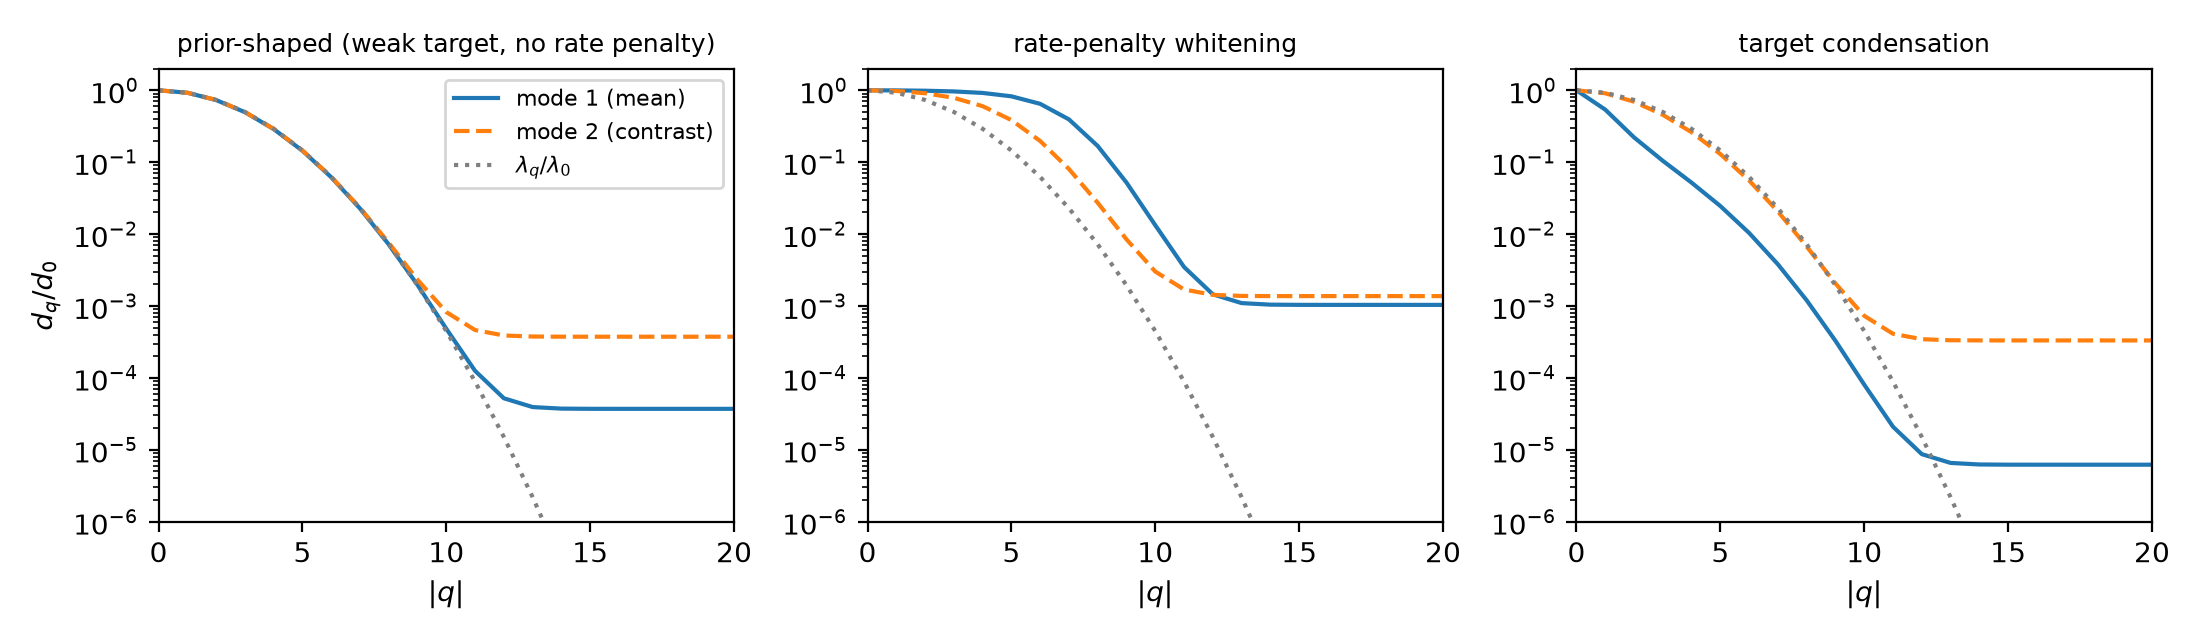
\includegraphics[width=\textwidth]{figures/linear_solution_limits_profiles.png}
  \caption{Normalised spectra $d_q/d_0$ of the mean direction (mode 1) and a contrast direction (mode 2) of the uniform latent task, ring $N = 64$, $\ell = 4$, $K = 3$, $a = 1$, $m = n = 8$, $P = 256$, $k_0 = k_1 = 1$, $\sigma^2 = 0.01$. Left: $r = 0$, $\beta = 0.25$ (P1): both follow $\lambda_q$ down to their noise floors. Middle: $r = 0.1$, $\beta = 0.25$ (P2): the stronger mode is whitened to higher $|q|$. Right: $r = 0$, $\beta = 10$ (P3): the stronger mode is pulled towards $q = 0$. Generated by \texttt{scripts/check\_linear\_soln\_limits.py}.}
  \label{fig:profiles}
\end{figure}

\subsection{The three regimes}
\label{sec:regimes}
Table~\ref{tab:regimes} lists the conditions. Each is tagged \task{} if it is set by $(Z, W_X, W_Y)$, \prior{} if by $(K, k_0, k_1, r, \sigma, \beta)$, and \mixed{} if by a product of the two.

\begin{table}[t]
  \centering
  \footnotesize
  \setlength{\tabcolsep}{4pt}
  \begin{tabular}{@{}>{\raggedright\arraybackslash}p{1.0cm}>{\raggedright\arraybackslash}p{2.0cm}>{\raggedright\arraybackslash}p{6.6cm}>{\raggedright\arraybackslash}p{3.4cm}>{\raggedright\arraybackslash}p{1.3cm}@{}}
    \toprule
    Regime & & Condition & Driver & Section \\
    \midrule
    \multicolumn{5}{@{}l}{\emph{(a) All latents share the same spatial profile}}\\
    (a1) & weak target, no penalty & $r = 0$, $\tau_k\ll1$ for all $k$: $d_q^{(k)} = \lambda_q\hat s_{X,k}^2 + \sigma^2$, the shape $\lambda_q$ above a common floor; $R_k(\Delta)/R_k(0)\to K(\Delta)$ for $\Delta\ge1$ when $\rho_k\gg1$ & \prior{} ($r$, $\beta$ small) & \ref{sec:r0} \\
    (a2) & zero temperature & $\sigma = r = 0$, $\Delta_k\ll1$ for all $k$: every mode has the same $\Theta$, hence the same $\tau(\Theta)$ and profile $\lambda_q/(1-\tau\ell_q^2)$, however strong the amplification & \prior{} ($\beta\to\infty$) given \task{} ($XX^\top\propto YY^\top$) & \eqref{eq:reduced} \\
    (a3) & equal singular values & the $K-1$ contrast modes always share a profile because their $s_k$ coincide; a statement about symmetry & \task{} (isotropic latents) & \ref{sec:latent} \\
    \addlinespace
    \multicolumn{5}{@{}l}{\emph{(b) Different latents separate across spatial scales} (both need unequal $s_k$)}\\
    (b1) & rate-penalty whitening & $\gamma_1\gg1+r\sigma^2\gg\gamma_2$, i.e.\ $\hat s_{X,2}^2\ll1/(r\lambda_0)\ll\hat s_{X,1}^2$, a window of width $3K+1$ in $r$; \emph{the stronger latent occupies finer scales} & \mixed{} ($r\lambda_0$ against $k_0s_k^2/m$) & \ref{sec:whiten} \\
    (b2) & target condensation & $\Delta_1\lesssim1\lesssim\Delta_2$, i.e.\ $\beta_c/(3K+1)\lesssim\beta\lesssim\beta_c = 12n\sqrt m/(\lambda_0\sqrt{k_0k_1}\,a^2)$ ($\beta\in[2.7,27]$ in Section~\ref{sec:predictions}); \emph{the stronger latent occupies coarser scales} & \mixed{} ($\beta$, $k_0k_1$, $\lambda_0$ against $a^2(3K+1)$, $n$, $m$) & \ref{sec:ring} \\
    \addlinespace
    \multicolumn{5}{@{}l}{\emph{(c) Nothing is spatially structured (white tuning maps)}}\\
    (c1) & noise-dominated & $\rho_k\ll1$, $\tau_k\ll1$: $d_q^{(k)} = \sigma_0^2(1+O(\rho_k))$; realised by $k_0\to0$, $\sigma\to\infty$ or small $P$ & \mixed{} ($k_0$, $\sigma$ against $s_k^2/m$) & Lem.~\ref{lem:floor} \\
    (c2) & rate-penalty clamp & $r\sigma^2\gg1$, $\tau_k\ll1$: $d_q\to1/r$ for every $q$, $k$ (at strong target $\amp_q$ still multiplies the clamp) & \prior{} & \ref{sec:whiten} \\
    (c3) & white prior & $\ell\to0$: $\lambda_q\equiv1$, no $q$-dependence at all & \prior{} & \ref{sec:r0} \\
    (c4) & null modes & anything outside $\col(Z)$ is white at level $\sigma_0^2$ & \task{} & Lem.~\ref{lem:floor} \\
    (c5) & full condensation & $\tau_k\to1$ for all $k$ with $\xi_k\gtrsim N$: every cell has the same tuning (uniform maps) & \mixed{} ($\Delta_k\ll1$, $\Theta\bar\ell_2\ll1$) & \ref{sec:ring} \\
    \bottomrule
  \end{tabular}
  \caption{Conditions for the three regimes of functional cell types, with the parameters that drive each. Both (b) mechanisms need unequal $s_k$: in the uniform task only mode 1 differs, by the factor $3K+1$. (a3) is the only purely task-driven statement in the list. Which direction (b) takes is decided by the prior: $r$ pushes a strong mode to fine scales, $\beta$ to coarse ones; the task only decides \emph{which} mode is strong.}
  \label{tab:regimes}
\end{table}

\paragraph{Mechanism (b1), whitening.} At weak target, $d_q^{(k)} - \sigma_0^2 = \lambda_q\hat s_{X,k}^2/\big[(1+r\sigma^2)(1+r\sigma^2 + r\lambda_q\hat s_{X,k}^2)\big]$. A mode with $\gamma_k\gg1+r\sigma^2$ is flat for $|q|$ below the crossover $\lambda_{q_k^\times} = (1+r\sigma^2)/(r\hat s_{X,k}^2)$ and follows $\lambda_q$ beyond; a mode with $\gamma_k\ll1$ follows $\lambda_q$ throughout (details in Section~\ref{sec:whiten}).

\paragraph{Mechanism (b2), condensation.} $\tau_k$ decreases with $\Delta_k\propto1/s_k^2$, so the mode with the largest $s_k$ is amplified first and its correlation length grows $\propto\hat s_{Y,k}$ while the others stay at $\ell$ (Section~\ref{sec:ring}); the window in $\beta$ follows from \eqref{eq:Delta-latent}.

\subsection{Rate-penalty whitening in detail}
\label{sec:whiten}
At weak target $d_q = \pi_q = \alpha_q/(1+r\alpha_q) = \frac1r - \frac{1}{r(1+r\alpha_q)}$, a saturating function of $\alpha_q$ capped at $1/r$. Subtracting the floor,
\begin{equation}
  d_q - \sigma_0^2 = \frac{\lambda_q\sX}{(1+r\sigma^2)\,(1+r\sigma^2 + r\lambda_q\sX)} ,
\end{equation}
which is $\propto\lambda_q$ when $r\lambda_q\sX\ll1+r\sigma^2$ and $\propto1$ (saturated) otherwise. A strong input mode fills its cap at the smooth frequencies and the latent-specific variance that distinguishes it from a weak mode sits at $|q|>q^\times$; relative to a weak mode, it is expressed at finer scales. Checked ($N = 64$, $\ell = 4$, $\sigma^2 = 0.01$, $r = 1$, $\delta = 50$): the formula holds to $4\times10^{-9}$, and the half-power frequency (defined as in Section~\ref{sec:predictions}, with $d_{N/2}$ as the floor) moves from $|q| = 3$ at $\gamma = 1$ to $|q| = 7$ at $\gamma = 100$ (script D2).

\section{Conditions to test numerically}
\label{sec:predictions}
Common setting unless stated: linear activation, one hidden layer on a ring of $N = 64$ sites, wrapped-Gaussian prior kernel \eqref{eq:ring} with $\ell = 4$ and $K_{i,i} = 1$, $m = n = 8$, $K = 3$ latents i.i.d.\ uniform on $[0,1]$ ($a = 1$), $P = 256$ patterns, $W_X$, $W_Y$ with orthonormal columns, $k_0 = k_1 = 1$, SGLD at inverse temperature $\beta$ (so $\delta = Pn/(\beta k_1) = 2048/\beta$), input noise $\sigma^2$, rate penalty $r$.

\paragraph{Measurement protocol.} After burn-in, for each posterior sample compute the $N\times P$ hidden activity $h$ and project it on $u_k$ (the eigenvectors of $ZZ^\top$: $u_1$ the mean direction, $u_2, u_3$ the contrasts, and the $P-3$ null directions) to get the tuning map $t_{i,k} = u_k^\top h_i$. Take the \emph{unitary} DFT over sites, $\tilde t_k(q) = N^{-1/2}\sum_i t_{i,k}e^{-2\pi\mathrm iqi/N}$ (the $F$ of Section~\ref{sec:start}), and average $|\tilde t_k(q)|^2$ over samples \emph{without subtracting the mean} across samples (the theory gives the second moment $\langle tt\rangle$ of \eqref{eq:tuning-map}) to get $\hat d_q^{(k)}$. From it: the half-power frequency $q^{(k)}_{1/2}$ (largest $|q|$ with $\hat d_q - \hat d_{N/2}\ge\frac12(\hat d_0 - \hat d_{N/2})$), the $q = 0$ share $\hat d_0/\sum_q\hat d_q$, and the lag-1 autocorrelation $R_k(1)/R_k(0)$. All predicted numbers are from script section E, which uses the same $\hat d_{N/2}$ floor; ``falsified'' thresholds allow for sampling error of order $10\%$. Each prediction is given as \emph{Setting} / \emph{Measure} / \emph{Predict} / \emph{Falsified if}. Predictions 4 and 5 need the activity noise $\eta$, which \path{fct} does not implement yet (see the closing paragraph).

\begin{enumerate}[leftmargin=2em,itemsep=4pt]
  \item \textbf{Prior-shaped maps (regime a1).}\\
  \emph{Setting:} $\sigma^2 = 0.01$, $r = 0$, $\beta = 0.25$.\\
  \emph{Measure:} $\hat d_q^{(1)}$, $\hat d_q^{(2)}$ and their ratio versus $q$; $q_{1/2}$; the $q = 0$ shares; $R_k(\Delta)/R_k(0)$ for $\Delta\le6$.\\
  \emph{Predict:} $\tau_1 = 0.008$, $\tau_2<10^{-3}$; $\hat d_q^{(k)} = \lambda_q\hat s_{X,k}^2 + \sigma^2$ with $\hat s_{X,1}^2 = 26.7$, $\hat s_{X,2}^2 = 2.67$; $q_{1/2} = 2$ for both modes, but only by a hair ($\lambda_3/\lambda_0 = 0.4996$), so a measured $q_{1/2} = 3$ is equally consistent; $q = 0$ share $0.157$ and $0.156$; $R_k(1)/R_k(0) = 0.969$ and $0.966$ ($\approx e^{-1/32}$); the ratio $\hat d_q^{(1)}/\hat d_q^{(2)}$ is about $10$ for $|q|\le8$, within $5\%$ ($10.08, 10.07, 10.04, 10.01, 10.00, 9.98, 9.95, 9.86, 9.56$ at $|q| = 0,\dots,8$), and then drops to the floor ratio $1.35$ by $|q| = 12$ ($8.54, 5.91, 2.73, 1.35$ at $|q| = 9,\dots,12$) as the contrast mode reaches its floor first.\\
  \emph{Falsified if} the two normalised spectra differ ($q_{1/2}$ by more than $1$, or the $q = 0$ shares by more than $0.03$), or the ratio varies by more than $20\%$ over $|q|\le8$, or $R_k(\Delta)/R_k(0)$ deviates from $e^{-\Delta^2/32}$ by more than $0.05$ for $\Delta\le6$.

  \item \textbf{Rate-penalty whitening (regime b1).}\\
  \emph{Setting:} as 1 but $r = 0.1$.\\
  \emph{Measure:} as 1.\\
  \emph{Predict:} $\gamma_1 = 26.7$, $\gamma_2 = 2.7$; $q_{1/2} = 6$ (mode 1) vs $4$ (mode 2); $q = 0$ share $0.077$ vs $0.111$; $R(1)/R(0) = 0.917$ vs $0.944$; the ratio $\hat d_q^{(1)}/\hat d_q^{(2)}$ is $1.32$ at $q = 0$ (down from $10$ in prediction 1: saturation), rises through $1.35, 1.44, 1.63, 2.02, 2.84, 4.35, 6.49$ at $|q| = 1,\dots,7$ to a peak of $8.2$ at $|q| = 8$--$9$ (mode 1 still on its $\lambda_q$ tail, mode 2 already near its floor), and is back at the floor ratio $1.35$ by $|q| = 12$ ($5.84, 2.72, 1.35$ at $|q| = 10, 11, 12$). It never reaches the $10$ of prediction 1.\\
  \emph{Falsified if} the mean direction's spectrum is not broader than the contrast's ($q^{(1)}_{1/2}\le q^{(2)}_{1/2}$), or $\hat d_0^{(1)}/\hat d_0^{(2)}>3$, or the ratio has no interior maximum above $4$.

  \item \textbf{Target condensation (regime b2).}\\
  \emph{Setting:} as 1 but $\beta = 10$; then the sweep $\beta = 0.25, 1, 2, 5, 10$.\\
  \emph{Measure:} $q = 0$ shares, $q_{1/2}$, $R(1)/R(0)$, $\hat d_0^{(1)}/\hat d_0^{(2)}$; the mode-1 and mode-2 shares along the sweep.\\
  \emph{Predict:} $\tau_1 = 0.83$, $\tau_2 = 0.11$; $q = 0$ share $0.343$ (mode 1) vs $0.164$ (mode 2); $q_{1/2} = 1$ vs $2$; $R(1)/R(0) = 0.985$ vs $0.967$; $\hat d_0^{(1)}/\hat d_0^{(2)} = 54$ ($\gg10$). Along the sweep the mode-1 share reads $0.157, 0.165, 0.188, 0.281, 0.343$ while mode 2 stays within $0.156$--$0.164$.\\
  \emph{Falsified if} mode 1's $q = 0$ share does not increase monotonically with $\beta$, if mode 2's share moves by more than $0.03$ over the sweep, or if $\hat d_0^{(1)}/\hat d_0^{(2)} < 20$ at $\beta = 10$.

  \item \textbf{White null modes (regime c4) and the floor level.}\\
  \emph{Setting:} $\sigma^2 = 1$, $r = 1$, $\beta = 0.25$, so $\sigma_0^2 = \sigma^2/(1+r\sigma^2) = 0.5$, a factor $2$ below the bare $\sigma^2$. Requires the activity noise $\eta$ (closing paragraph): without it the hidden activity of a linear network lies exactly in $\col(Z)$, every null direction has identically zero power, and the floor does not exist; that zero is the $\sigma\to0$ statement (i) of Section~\ref{sec:sigma0} and checks the projection, not the theory.\\
  \emph{Measure:} $\hat d_q$ of the $253$ null directions and of the two latent modes; $R(\Delta)/R(0)$.\\
  \emph{Predict:} every null direction has a flat spectrum at $0.5$ and $|R(\Delta)/R(0)|<0.05$ for $\Delta\ge1$; the latent modes sit above it with $\hat d_0/\sigma_0^2 = 2.0$ and $1.9$ and $R(1)/R(0) = 0.18$ and $0.14$.\\
  \emph{Falsified if} the null-direction autocorrelation at $\Delta = 1$ exceeds $0.1$, or its level differs from $0.5$ by more than a factor $1.5$ (which excludes the bare $\sigma^2 = 1$).

  \item \textbf{Noise-dominated (regime c1).}\\
  \emph{Setting:} $k_0 = 0.001$, $\sigma^2 = 1$, $r = 0$, $\beta = 0.25$ ($\rho_1 = 0.3$). Requires $\eta$, as 4.\\
  \emph{Measure:} $\hat d_0/\hat d_{N/2}$ and $R(1)/R(0)$ for both modes.\\
  \emph{Predict:} $\hat d_0/\sigma_0^2 = 1.27$ (mode 1) and $1.03$ (mode 2); $R(1)/R(0) = 0.025$ and $0.003$: all tuning maps white.\\
  \emph{Falsified if} any $R_k(1)/R_k(0)>0.15$ or $\hat d_0^{(1)}/\hat d_{N/2}^{(1)}>2$.

  \item \textbf{No individual-latent cell types (Section~\ref{sec:latent}, remark 2).}\\
  \emph{Setting:} any of 1--3.\\
  \emph{Measure:} the tuning of each neuron in each sample to the \emph{orthonormal} contrast pair $(u_2, u_3)$ only, the angle $\theta_i = \operatorname{atan2}(t_{i,3}, t_{i,2})$, and $\langle\cos4\theta_i\rangle$ over neuron-samples.\\
  \emph{Predict:} the joint distribution of $(t_{i,2}, t_{i,3})$ is rotation-invariant, so $\theta_i$ is uniform on the circle and $\langle\cos4\theta_i\rangle = 0$; an axis-aligned population gives a positive value. The reference pair matters: an isotropic cloud seen in an oblique frame is squeezed along the frame's bisector, so tuning to a non-orthogonal pair such as the raw or pattern-centred $(z_2, z_3)$ (correlated through the shared mean) gives a \emph{negative} value under the null (of order $-0.1$ in a quick projection check outside the script; the exact value depends on how the tuning is normalised), which would be mistaken for a diagonal population. The test is meaningful only in the orthonormal frame.\\
  \emph{Falsified if} $|\langle\cos4\theta\rangle|>0.1$ in the frame $(u_2, u_3)$ with more than $10^3$ neuron-samples. A violation would be the most informative outcome: it would show that cell types aligned to individual latents arise from something outside the linear Gaussian theory (non-linearity, finite $N$, or SGLD not at equilibrium).

  \item \textbf{Correlation length tracks the prior.}\\
  \emph{Setting:} 1 with $\ell\in\{2,4,8\}$.\\
  \emph{Measure:} $R_k(\Delta)/R_k(0)$ for $1\le \Delta\le2\ell$ and $R_k(0)$, both modes.\\
  \emph{Predict:} $R_k(\Delta)/R_k(0) = K(\Delta)$, the wrapped Gaussian of \eqref{eq:ring} (indistinguishable from $e^{-\Delta^2/2\ell^2}$ at these $\ell$), to within $7\times10^{-3}$ for $\Delta\le2\ell$ (the small deviations are the floor and the target amplification); the Gaussian width read off at $\Delta = \ell$ is $2.00, 4.01, 8.06$ for mode 1 and $1.99, 3.99, 7.97$ for mode 2. $R_k(0) = \hat s_{X,k}^2 + \sigma^2$ is nearly independent of $\ell$ because $\bar\lambda = 1$: $26.7, 26.8, 27.2$ for mode 1 (the $1.7\%$ rise at $\ell = 8$ is the growing target amplification, $\tau_1\propto\lambda_0\propto\ell$) and $2.677$ for mode 2 at every $\ell$ (script E, P7).\\
  \emph{Falsified if} the fitted Gaussian width differs from $\ell$ by more than $20\%$, or $R_k(0)$ changes by more than $15\%$ across $\ell$.

  \item \textbf{A common prior scale is non-monotone (Section~\ref{sec:k}).}\\
  \emph{Setting:} 3 ($\sigma^2 = 0.01$, $r = 0$, $\beta = 10$) with $k_0 = k_1 = k\in\{0.01, 0.1, 1, 10, 100\}$.\\
  \emph{Measure:} the $q = 0$ share of both modes at each $k$.\\
  \emph{Predict:} mode-1 share 0.152, 0.166, 0.343, 0.166, 0.157 (peak at $k = 1$); mode 2: 0.118, 0.152, 0.164, 0.165, 0.157.\\
  \emph{Falsified if} the mode-1 share is monotone in $k$ or its peak value is below $0.25$.
\end{enumerate}

\paragraph{What \texttt{fct} does not yet match.}
The numbers above assume the notes' model as stated. Four conventions differ in the \path{fct} code, and the follow-up item that maps these predictions onto \path{fct} has to resolve each:
\begin{enumerate}[nosep]
  \item \emph{Centred latents.} \path{fct/tasks.py} draws $z_k$ uniform on $[-a,a]$: no mean direction, all $K$ modes degenerate at $s^2 = Pa^2/3$. Predictions 1--3 and 8 use the mean direction as the strong mode; with centred latents every mode has the same spectrum, and only 4--7 carry over unchanged (with $u_1,u_2,u_3$ any orthonormal basis of $\col(Z)$).
  \item \emph{Gaussian teacher.} $W_X$ and $W_Y$ have i.i.d.\ $\mathcal N(0,1/K)$ entries rather than orthonormal columns, so the ansatz is approximate (Section~\ref{sec:rederive}: $0.2\%$ on $c$ for a mild skew).
  \item \emph{No activity noise.} The notes' first layer carries $\eta^\mu_i\sim\mathcal N(0,\sigma^2)$ per pattern and neuron (\texttt{eq:ff-network}, integrated out in \texttt{eq:single-site-reg}); the forward pass of \path{fct/model.py} is deterministic, and its parameter \texttt{g} is the gain $g/\sqrt N$ on the recurrent weights, not a rate penalty. Without $\eta$ the activity $h^{(1)} = W^{(0)}X^\top/\sqrt m$ of a linear layer lies exactly in $\col(Z)$: the null-direction power and the floor $\sigma_0^2$ of Lemma~\ref{lem:floor} are entirely $\eta$'s, so predictions 4 and 5 are untestable as the code stands and the $\sigma^2$ of 1--3 and 7 must be read as $0$ (the limit of Section~\ref{sec:sigma0}, regular for the latent modes). Implementing $\eta$ means adding $\sigma\xi^\mu_i$, $\xi\sim\mathcal N(0,1)$ drawn fresh per $(\mu,i)$, to $h^{(1)}$ at every forward pass during sampling.
  \item \emph{Rate penalty.} The notes' loss carries $\frac1\beta\mathcal P_{\mathrm{rates}} = \frac1{2\beta}\sum_{l,\mu,i,j}\phi^{(l)\mu}_iG^{(l)}_{i,j}\phi^{(l)\mu}_j$ with $G^{(l)} = rI$, i.e.\ $\frac{r}{2\beta}\sum\phi^2$; \path{fct/train.py} adds $\texttt{rate\_lambda}\sum_{l,\mu,i}\phi(h^{(l)\mu}_i)^2$ to a loss whose data term $\frac N2\,\mathrm{mse}$ equals the notes' $\frac N{2Pn}\sum(f-y)^2$, and samples $e^{-\beta L}$. The two agree with $\texttt{rate\_lambda} = r/(2\beta)$ (the \texttt{rate\_tilt} $= 2\beta\,\texttt{rate\_lambda}$ of \path{docs/design.md} is $r$), with \texttt{train.beta} the notes' $\beta$.
\end{enumerate}

\appendix
\section{Reproducing the numbers}
From the repository root, \texttt{uv run python} \path{latex/notes/scripts/check_linear_soln_limits.py} (a few seconds) prints sections A--E quoted above and writes \path{latex/notes/figures/linear_solution_limits_profiles.png}. All parameters are module constants at the top of the script; the random seed is $0$.
\end{document}
